\documentclass{article}\usepackage{graphicx, color}
%% maxwidth is the original width if it is less than linewidth
%% otherwise use linewidth (to make sure the graphics do not exceed the margin)
\makeatletter
\def\maxwidth{ %
  \ifdim\Gin@nat@width>\linewidth
    \linewidth
  \else
    \Gin@nat@width
  \fi
}
\makeatother

\definecolor{fgcolor}{rgb}{0.2, 0.2, 0.2}
\newcommand{\hlnumber}[1]{\textcolor[rgb]{0,0,0}{#1}}%
\newcommand{\hlfunctioncall}[1]{\textcolor[rgb]{0.501960784313725,0,0.329411764705882}{\textbf{#1}}}%
\newcommand{\hlstring}[1]{\textcolor[rgb]{0.6,0.6,1}{#1}}%
\newcommand{\hlkeyword}[1]{\textcolor[rgb]{0,0,0}{\textbf{#1}}}%
\newcommand{\hlargument}[1]{\textcolor[rgb]{0.690196078431373,0.250980392156863,0.0196078431372549}{#1}}%
\newcommand{\hlcomment}[1]{\textcolor[rgb]{0.180392156862745,0.6,0.341176470588235}{#1}}%
\newcommand{\hlroxygencomment}[1]{\textcolor[rgb]{0.43921568627451,0.47843137254902,0.701960784313725}{#1}}%
\newcommand{\hlformalargs}[1]{\textcolor[rgb]{0.690196078431373,0.250980392156863,0.0196078431372549}{#1}}%
\newcommand{\hleqformalargs}[1]{\textcolor[rgb]{0.690196078431373,0.250980392156863,0.0196078431372549}{#1}}%
\newcommand{\hlassignement}[1]{\textcolor[rgb]{0,0,0}{\textbf{#1}}}%
\newcommand{\hlpackage}[1]{\textcolor[rgb]{0.588235294117647,0.709803921568627,0.145098039215686}{#1}}%
\newcommand{\hlslot}[1]{\textit{#1}}%
\newcommand{\hlsymbol}[1]{\textcolor[rgb]{0,0,0}{#1}}%
\newcommand{\hlprompt}[1]{\textcolor[rgb]{0.2,0.2,0.2}{#1}}%

\usepackage{framed}
\makeatletter
\newenvironment{kframe}{%
 \def\at@end@of@kframe{}%
 \ifinner\ifhmode%
  \def\at@end@of@kframe{\end{minipage}}%
  \begin{minipage}{\columnwidth}%
 \fi\fi%
 \def\FrameCommand##1{\hskip\@totalleftmargin \hskip-\fboxsep
 \colorbox{shadecolor}{##1}\hskip-\fboxsep
     % There is no \\@totalrightmargin, so:
     \hskip-\linewidth \hskip-\@totalleftmargin \hskip\columnwidth}%
 \MakeFramed {\advance\hsize-\width
   \@totalleftmargin\z@ \linewidth\hsize
   \@setminipage}}%
 {\par\unskip\endMakeFramed%
 \at@end@of@kframe}
\makeatother

\definecolor{shadecolor}{rgb}{.97, .97, .97}
\definecolor{messagecolor}{rgb}{0, 0, 0}
\definecolor{warningcolor}{rgb}{1, 0, 1}
\definecolor{errorcolor}{rgb}{1, 0, 0}
\newenvironment{knitrout}{}{} % an empty environment to be redefined in TeX

\usepackage{alltt}
\usepackage{amsmath}
\usepackage{natbib}
\title{Notes on VAR Analysis for Doctorate}
\author{Rob Hayward}
\IfFileExists{upquote.sty}{\usepackage{upquote}}{}

\begin{document}
\maketitle

\section{Preparation of data}
The preparation of data is straight forward.  The figures are downloaded and adjustments are made.  It is possible to chose from a number of options for the data to be analysed in the VAR. 
\begin{itemize}
\item The full dataset includes CNB, CNE, CNFDI, RTWI, SPREAD1 and SPREAD2 as well as S1 and S2.  
\item There are three dummy variables
\item The data can be normalised to deal with the issue of hetorscedasticity that is evident in some of the series
\item The current account can be added.  
\item It is possible to consider breaks in the data to deal with the issue of parameter instability. This can take three forms: 
\begin{itemize}
\item Select a break period and check the stability of parameters before and after the break
\item Impose an intervention dummy after the break and check statistical significance. 
\item Look at rolling estimates of the parameters to assess stability
\end{itemize}
\end{itemize}

These can all be tested for unit roots to begin and as cointegrated vectors as a second move.  The labtop has a loop to calcualte the Augmented Dickey-Fuller tests of the key variables. 

\section{Unit roots}

The $\tau_3$ test statistic is the test of the null hypothesis that the coefficient on the difference of the lagged dependent variable is equal to zero and that there is a \emph{unit root} as $\rho$ is equal to one.  


The critical value for a sample size of 100 comes from \citep{Fuller1976}. 

An F-test of the null hypothesis that the coefficients on the lagged change in the dependend variable and the coefficient on the time trend are jointly equal to zero is also supplied $(\phi_3)$.  The critical values come from Table VI \citep{DF1981} testing the null $(\alpha, \beta, \rho) = (\alpha, 0, 1)$.  It seems that unit root and lack of time trend cannot be rejected. A joint test of the null that the coefficients on the drift, time trend and lagged difference of the dependent variable is suppoed in $(\phi_2)$.  The critical values come from Table V \citep{DF1981} testing the null $(\alpha, \beta, \rho) = (0, 0, 1)$.
\begin{knitrout}
\definecolor{shadecolor}{rgb}{0.969, 0.969, 0.969}\color{fgcolor}\begin{kframe}


{\ttfamily\noindent\bfseries\color{errorcolor}{\#\# Error: object 'd' not found}}

{\ttfamily\noindent\bfseries\color{errorcolor}{\#\# Error: object 'd' not found}}

{\ttfamily\noindent\bfseries\color{errorcolor}{\#\# Error: object 'd' not found}}

{\ttfamily\noindent\bfseries\color{errorcolor}{\#\# Error: object 'd' not found}}

{\ttfamily\noindent\bfseries\color{errorcolor}{\#\# Error: object 'd' not found}}

{\ttfamily\noindent\bfseries\color{errorcolor}{\#\# Error: object 'd' not found}}

{\ttfamily\noindent\bfseries\color{errorcolor}{\#\# Error: object 'd' not found}}\end{kframe}
\end{knitrout}


\begin{kframe}


{\ttfamily\noindent\bfseries\color{errorcolor}{\#\# Error: could not find function "ur.df"}}\end{kframe}% latex table generated in R 2.15.2 by xtable 1.7-0 package
% Thu Jun 27 22:16:04 2013
\begin{table}[ht]
\begin{center}
\begin{tabular}{rrrrrrrr}
  \hline
 & CNB & CNE & CNFDI & COT & RTWI & SPREAD2 & S1 \\ 
  \hline
tau & 0.00 & 0.00 & 0.00 & 0.00 & 0.00 & 0.00 & 0.00 \\ 
  CV(tau) & 0.00 & 0.00 & 0.00 & 0.00 & 0.00 & 0.00 & 0.00 \\ 
  phi2 & 0.00 & 0.00 & 0.00 & 0.00 & 0.00 & 0.00 & 0.00 \\ 
  CV(phi) & 0.00 & 0.00 & 0.00 & 0.00 & 0.00 & 0.00 & 0.00 \\ 
   \hline
\end{tabular}
\end{center}
\end{table}

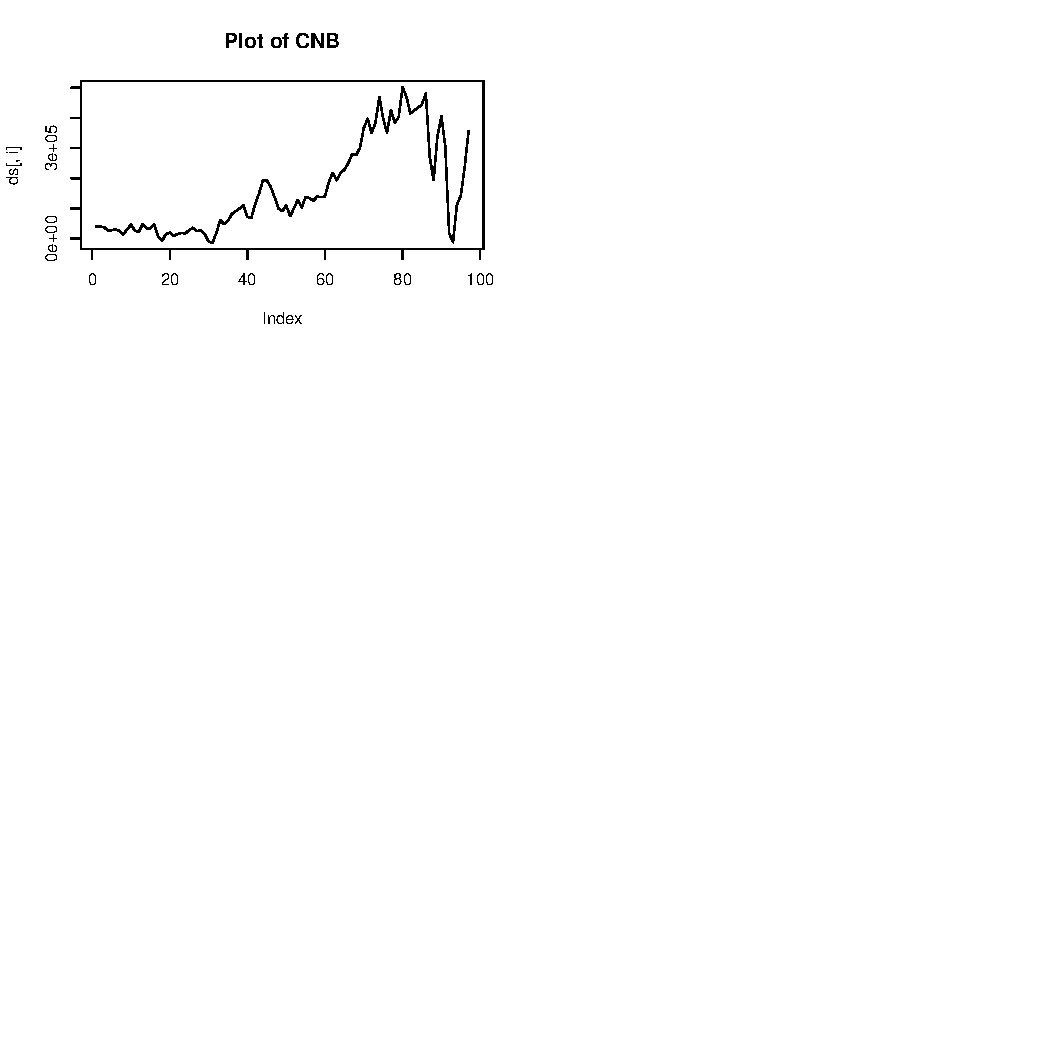
\includegraphics[width=\maxwidth]{figure/ur} 



\section{Cointegration tests with capital flow data}
Testing for cointegration of the series.  For the F-Test, that the coefficient on the lagged difference of the dependent variable and the coefficient on the It appears that the null of a unit root cannot be rejected for CNB, RTWI, Spread2. It is rejected at the 5\% level for CNE, CFDI, COT and S1.  Therefore, it appears that the former should be introduced in first difference. 



According to the results from the "Test type: maximal eigenvalue statistic (lambda max), with linear trend in cointegration", there are 3 or 4 cointegrating realtionships.  


The next step would be to use the cajorls function to estimate an errror correction model. The results of this activity are shown in the following table.

\begin{tabular}{l | r r r r}
test  & 10pct   &   5pct &   1pct & test stat\\
\hline
r <= 6 &   1.91 &  6.50  & 8.18   & 11.65\\
r <= 5 &  13.07 & 15.66  & 17.95  & 23.52\\
r <= 4 &  31.44 & 28.71  & 31.52  & 37.22\\
r <= 3 &  59.99 & 45.23  & 48.28  & 55.43\\
r <= 2 & 106.41 & 66.49  & 70.60  & 78.87\\
r <= 1 & 168.18 & 85.18  & 90.39  & 104.20\\
r = 0  & 251.31 & 118.99 & 124.25 & 136.06\\
\end{tabular}

This suggests that there are three or four conintegrating variables.  The results are the same no matter what the combination that is adopted.  

\end{document}
